\chapter{Análise de Variabilidade Conjunta (MEOF)}
\label{chap:meof}

Após caracterizar separadamente a precipitação e o vento nos capítulos anteriores, este capítulo avalia sua simultaneidade espaço-temporal mediante a Análise de Funções Ortogonais Empíricas Multivariadas (MEOF), que integra o vento a 10 metros e a precipitação total para identificar os modos dominantes de variabilidade conjunta.
Diferentemente da análise univariada, a decomposição MEOF expõe a geometria da covariabilidade entre a circulação atmosférica e o campo de precipitação, permitindo determinar se seus padrões principais covariam no mesmo setor do domínio centrado no sistema ou respondem a dinâmicas diferenciadas.

\section{Fracionamento da Variância Conjunta}
\label{sec:meof_varianza}

A Figura~\ref{fig:all_expvar_meof} apresenta o espectro de variância conjunta explicada pelos cinco primeiros modos multivariados (MEOF1 a MEOF5), contrastando a População Global (painel a) com o subconjunto de alta vorticidade (p90, painel b) para as combinações de região de ciclogênese (SBR, LPB, ARG) e fase evolutiva.
Esta figura foi obtida aplicando o MEOF sobre a matriz padronizada de anomalias conjuntas de ambas as variáveis (Seção~\ref{subsec:eof_multivariado}), com o fim de quantificar a dimensionalidade da covariabilidade entre vento e precipitação, e estabelecer se a covariância se concentra em um padrão dominante ou se distribui entre múltiplos modos competitivos.

Na População Global, o MEOF1 capta entre 14.8\% e 26.6\% da variância conjunta segundo fase e região, com queda progressiva em direção aos modos secundários, um valor intermediário entre o EOF1 univariado do vento (30.9--57.4\%, Seção~\ref{sec:var_exp_wind10}) e o da precipitação (11--16\%, Seção~\ref{subsec:var_exp_tp}).
Esse espectro relativamente concentrado, embora menos dominante do que o EOF1 univariado do vento, indica que nos ciclones ordinários ambas as variáveis covariam de forma moderada em um único padrão espacial de grande escala, compatível com a organização frontal do WCB, que estruturaria simultaneamente a banda de precipitação e o gradiente de vento no flanco quente do sistema (essa interpretação é examinada com mais detalhe na Seção~\ref{sec:discusion_meof}, onde se avalia quanto cada campo contribui ao modo conjunto).
No subconjunto de alta vorticidade (p90), por sua vez, a variância explicada pelo MEOF1 cai para valores mais baixos, com um mínimo de 11.65\% em ARG durante a intensificação e um máximo de 23.47\% em LPB durante o decaimento.
Essa redução e o achatamento do espectro em direção aos modos secundários indicam, segundo \citet{hannachi2007empirical}, que o sistema é mais complexo e multidimensional quando os autovalores estão mais próximos entre si. Isso poderia refletir que, nos sistemas p90, várias configurações de covariabilidade competem em importância, por exemplo a CCB frente às bandas convectivas do setor quente, ou a intrusão seca frente ao WCB, sem que nenhum padrão único capture mais do que uma fração minoritária da covariância total.

\begin{figure}[htbp]
    \centering
    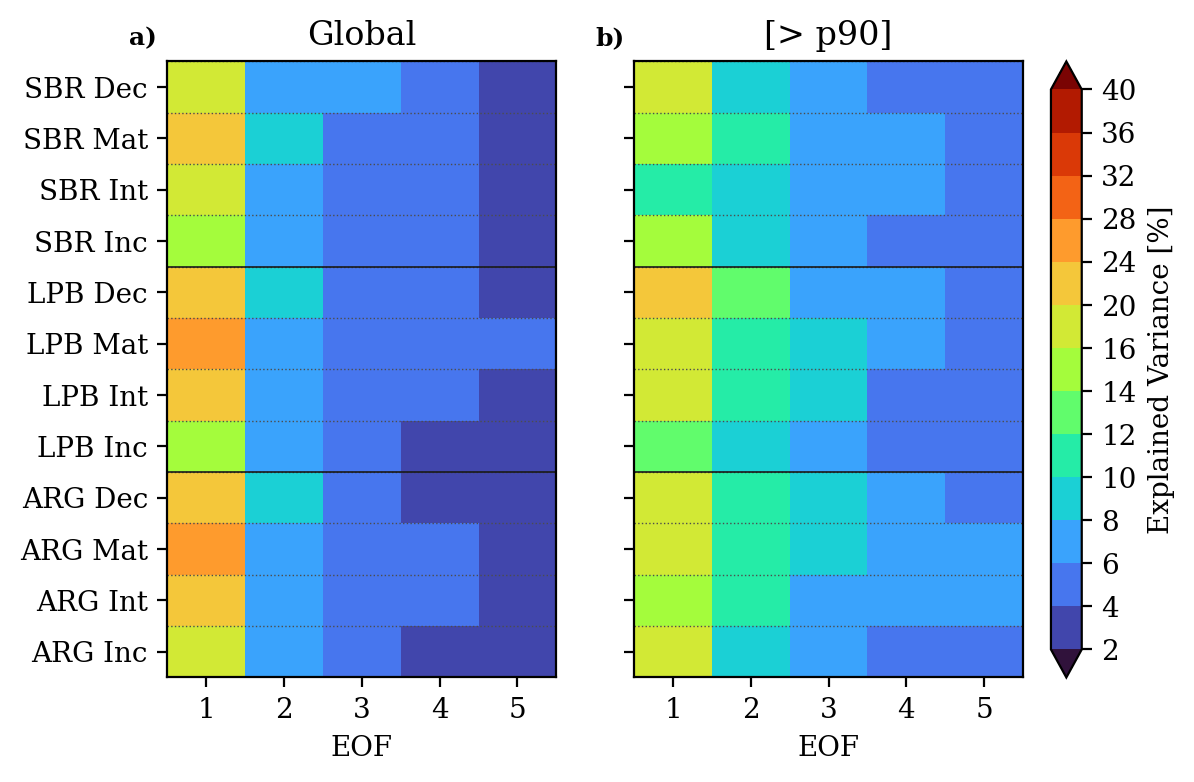
\includegraphics[width=0.8\textwidth]{images/meof/all_expvar_meof.png}
    \caption[Variância conjunta explicada pelos modos conjuntos (MEOF1--MEOF5)]{Fracionamento da variância conjunta total contida nos primeiros cinco modos espaciais multivariados (MEOF1 a MEOF5). Contrasta-se a distribuição da covariância entre o vento a 10 metros e a precipitação para a População Global (painel a) frente ao subconjunto de alta vorticidade (p90, painel b). As barras de cada linha representam as combinações de região de ciclogênese e fase evolutiva.}
    \label{fig:all_expvar_meof}
\end{figure}

\section{Evolução dos Padrões Espaciais Conjuntos (MEOF1)}
\label{sec:meof_patrones}

Os padrões espaciais do primeiro modo multivariado (MEOF1) revelam como se organiza a covariância de vento e precipitação no domínio centrado no sistema à medida que o ciclone evolui.
A análise se concentra em duas fases diagnosticamente centrais: a intensificação, onde se estabelece a configuração conjunta inicial, e a maturidade, onde a reorganização espacial entre variáveis alcança sua expressão mais marcada nos sistemas p90.

A seleção dessas duas fases, em vez das quatro que compõem o ciclo de vida (Seção~\ref{subsec:tb_fases}), obedece a duas razões.
Por um lado, a fase incipiente corresponde por definição ao surgimento inicial de uma circulação organizada, quando os sistemas ainda exibem circulações assimétricas antes de consolidar uma circulação fechada e apresentam uma variabilidade de intensidade inter-sistêmica marcadamente maior do que nas fases posteriores; essa heterogeneidade, já evidenciada na baixa e dispersa variância explicada pelo EOF1 univariado durante a incipiência (Seções~\ref{sec:var_exp_wind10} e~\ref{subsec:var_exp_tp}), reflete que a diversidade de configurações responde não apenas à região de ciclogênese mas também à falta de organização morfológica dos sistemas, o que limita a interpretabilidade física de um modo conjunto dominante.
Por outro lado, a fase de decaimento tem menor relevância prática. Os ciclones do Atlântico Sul-Ocidental deslocam sua trajetória preferencialmente em direção ao sudeste e ao oceano aberto, de modo que no decaimento a maioria dos sistemas já se encontra afastada do litoral sul-americano.
Por essas razões, a análise detalhada do MEOF1 se concentra em intensificação e maturidade, as fases onde a covariabilidade entre ambos os campos é estatisticamente mais interpretável.

\subsection{Fase de Intensificação}
\label{subsec:meof_intensificacion}

A Figura~\ref{fig:meof_intensificacion_global} apresenta o primeiro modo espacial multivariado (MEOF1) durante a intensificação para a População Global.
Cada linha corresponde a uma região de ciclogênese (SBR, LPB e ARG) e cada grupo de colunas mostra os padrões MEOF1 de precipitação (coluna esquerda) e vento a 10 metros (coluna central), junto com o índice da componente principal (PC1, coluna direita).
A escala cromática divergente quantifica as anomalias padronizadas do MEOF1, com tons vermelhos para cargas positivas e azuis para negativas no domínio centrado no sistema. A variância explicada, indicada sobre cada painel de PC1, oscila entre 18.99\% (ARG) e 22.92\% (LPB).
Esta figura é construída aplicando o MEOF sobre a matriz padronizada de anomalias conjuntas de ambas as variáveis no domínio centrado no sistema, com o fim de estabelecer o padrão de referência do desenvolvimento baroclínico padrão durante o período de intensificação do sistema na climatologia média.

\begin{figure}[htbp]
    \centering
    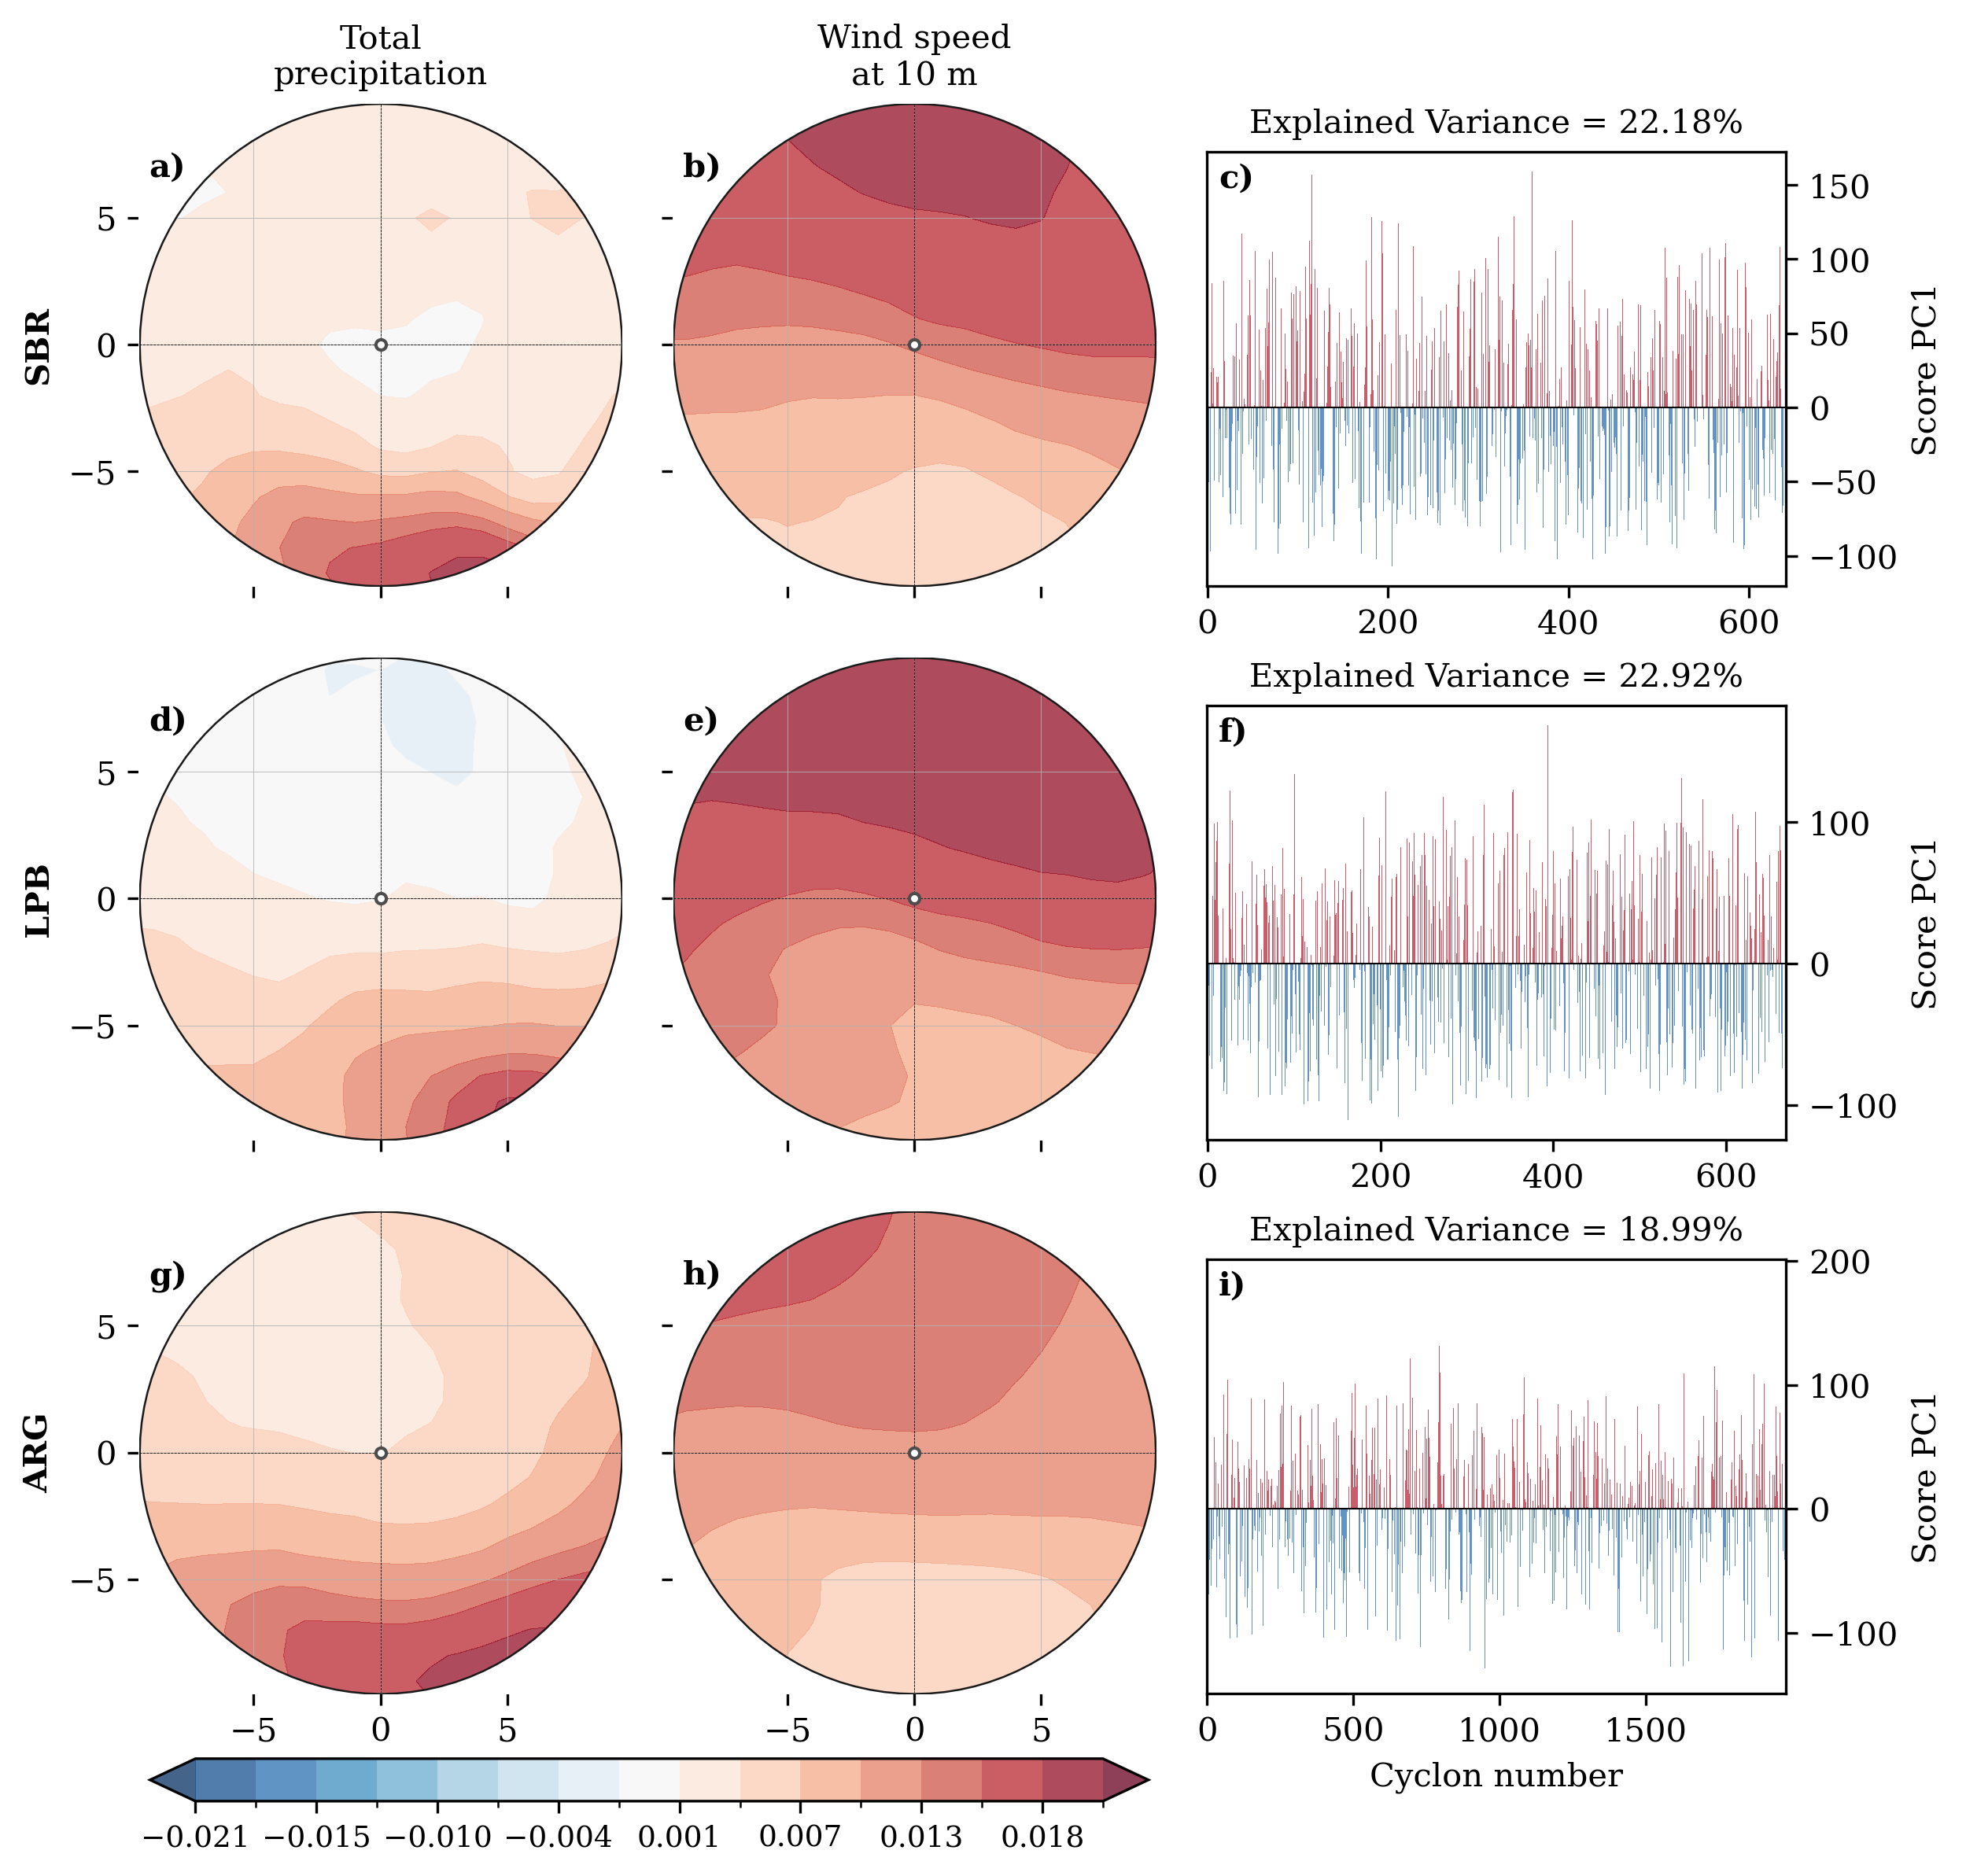
\includegraphics[width=\textwidth]{images/meof/meof1_intensification_global.png}
    \caption[MEOF1 de vento a 10 m e precipitação -- Intensificação (População Global)]{Primeiro modo espacial multivariado (MEOF1) durante a fase de intensificação para a População Global. As colunas mostram, para cada região (SBR: linhas a--c; LPB: linhas d--f; ARG: linhas g--i), os padrões MEOF1 de precipitação total (coluna esquerda), vento a 10 m (coluna central) e o índice da PC1 (coluna direita). A variância conjunta explicada é indicada sobre cada painel de PC1. A escala cromática divergente quantifica as anomalias padronizadas do MEOF1 no domínio centrado no sistema de $20^{\circ} \times 20^{\circ}$.}
    \label{fig:meof_intensificacion_global}
\end{figure}

Durante a intensificação, a População Global apresenta um padrão de covariância consistente nas três regiões, embora com matizes regionais. O campo de precipitação (painéis a, d, g) mostra anomalias positivas fracas na maior parte do domínio, com o núcleo mais definido em direção ao sul e sudeste do vórtice (até $+0.018$ em SBR e LPB); em SBR (a) e LPB (d) esse sinal se concentra em um foco compacto no quadrante sul, enquanto em ARG (g) se distribui de forma mais difusa sobre boa parte do domínio, sem um núcleo tão marcado. O campo de vento (painéis b, e, h), por sua vez, apresenta anomalias positivas muito mais intensas e estendidas, dominando a metade norte do domínio nas três regiões, particularmente em LPB (e), onde a carga positiva cobre quase todo o semicírculo norte, com valores muito altos, próximos do limite superior da escala, e decrescendo gradualmente em direção ao sul sem mudar de sinal. A correlação entre essa carga e o EOF1 univariado de cada campo (Seção~\ref{sec:discusion_meof}) mostra que, nessa fase, tanto o vento ($|r|=0.99$ a $1.00$) quanto a precipitação ($|r|=0.72$ a $0.95$) coincidem fortemente com seus próprios padrões univariados.

A Figura~\ref{fig:meof_intensificacion_p90} apresenta os mesmos padrões do MEOF1 durante a intensificação, restrita ao subconjunto de ciclones de alta vorticidade (p90).
Com disposição de painéis idêntica à figura precedente, seu propósito é documentar a primeira reorganização estrutural da covariabilidade que antecipa a diferenciação espacial completa que se consolidará na maturidade.
A variância explicada desce para valores de 11.65\% (ARG), 17.03\% (LPB) e 14.06\% (SBR), refletindo a dispersão da covariância em direção a modos secundários.

O contraste com a População Global é imediato e profundo. O campo de precipitação (painéis a, d, g) perde por completo a extensão difusa do padrão global e desenvolve uma estrutura multilobular. Em SBR (painel a) aparece um núcleo de anomalias positivas intensas e compactas ($>+0.013$) próximo do vórtice, ligeiramente deslocado para leste e para o sul ($\Delta x \approx +1^{\circ}$ a $+3^{\circ}$, $\Delta y \approx -0.5^{\circ}$ a $-2^{\circ}$), flanqueado por dois lóbulos de anomalias negativas, um a nordeste e outro ao sul, configurando já uma estrutura assimétrica de lóbulos diferenciados.
Em LPB (painel d), o padrão de precipitação mostra uma faixa de anomalias positivas com inclinação noroeste-sudeste, com o núcleo mais intenso próximo do vórtice e uma extensão secundária em direção ao noroeste, flanqueada por anomalias negativas concentradas a nordeste e, em menor medida, ao sul.
Em ARG (painel g), o núcleo positivo de precipitação é o mais intenso e compacto dos três, centrado sobre o vórtice e estendido em direção ao leste ($\Delta x \approx 0^{\circ}$ a $+5^{\circ}$, $\Delta y \approx -2^{\circ}$ a $+1^{\circ}$), com uma carga que supera o limite superior da escala ($>0.0208$) no máximo, e com anomalias negativas fracas a oeste e a nordeste.
O campo de vento (painéis b, e, h) exibe um comportamento distinto. Nas três regiões, as anomalias são negativas na maior parte do domínio, mais intensas em direção ao norte, com uma faixa de valores neutros ou levemente positivos ao sul do vórtice, onde em LPB e ARG chega até a se tornar fracamente positiva.
Esse padrão, vento que se intensifica negativamente em direção ao norte enquanto a precipitação se concentra perto do vórtice e em direção ao sul, revela já o germe da separação de quadrantes. Os máximos de precipitação e vento não covariam positivamente, mas o MEOF1 captura uma configuração de anticovariância incipiente, com o forçamento pluviométrico se concentrando onde o forçamento eólico é mais fraco. Essa mesma comparação confirma que, em p90, o vento também ancora quase por completo o modo conjunto ($|r|=0.96$ a $1.00$), exceto em ARG, onde a precipitação já contribui com covariância genuína desde essa fase ($|r|=0.92$), diferentemente de SBR e LPB ($|r|=0.08$--$0.20$), que só alcançam esse nível na maturidade (Seção~\ref{sec:discusion_meof}).

\begin{figure}[htbp]
    \centering
    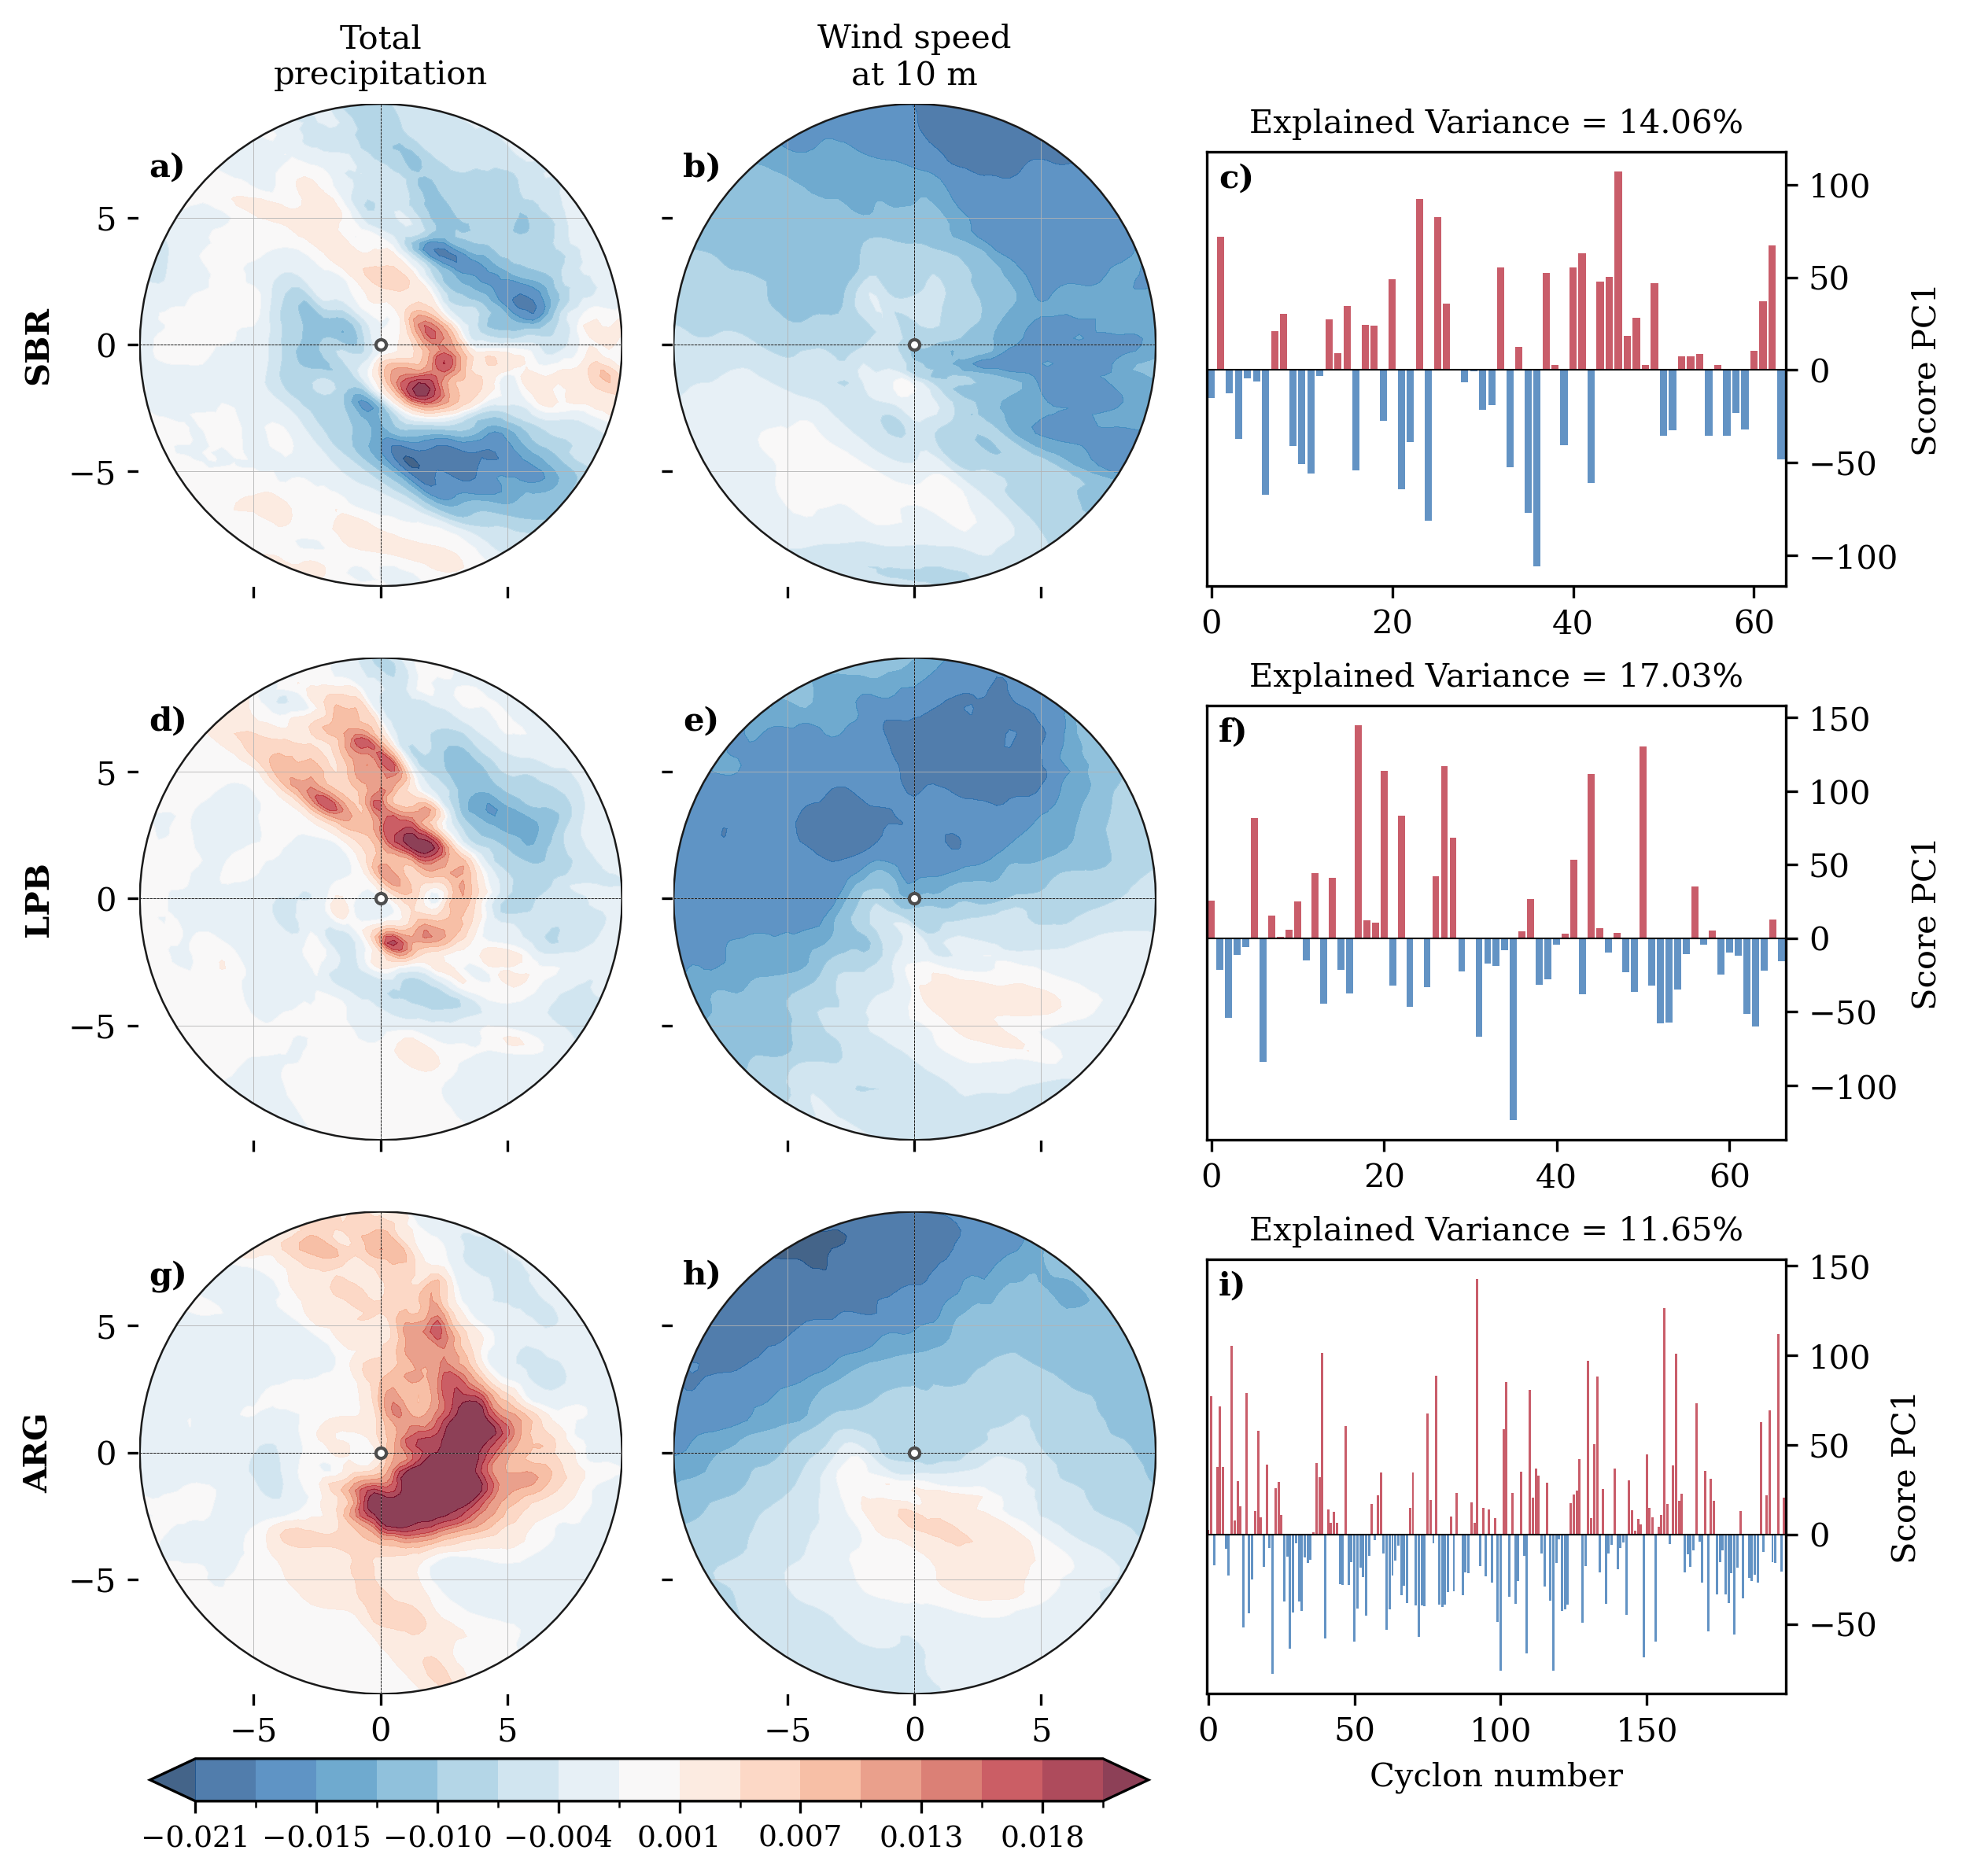
\includegraphics[width=\textwidth]{images/meof/meof1_intensification_p90.png}
    \caption[MEOF1 de vento a 10 m e precipitação -- Intensificação (p90)]{Primeiro modo espacial multivariado (MEOF1) durante a fase de intensificação para o subconjunto de ciclones de alta vorticidade (p90). O formato de painéis, a escala cromática e o domínio são idênticos à Figura~\ref{fig:meof_intensificacion_global}, permitindo quantificar a contração da covariância e a emergência da assimetria estrutural durante o desenvolvimento do sistema.}
    \label{fig:meof_intensificacion_p90}
\end{figure}

A emergência da assimetria já durante a intensificação nos sistemas p90 poderia ter uma explicação física.
Durante a intensificação baroclínica ativa, a precipitação se organiza na ascensão frontal do WCB no flanco quente-oriental do ciclone, enquanto a CCB emergente dá forma à nebulosidade da \textit{cabeça da vírgula} \citep{browning1986conceptual} e começa a envolver o núcleo do sistema.
Em ciclones ordinários, esses dois processos operam de maneira suave e parcialmente superposta, gerando a covariância difusa documentada na População Global.
Nos sistemas intensos, essa separação poderia ocorrer já durante a própria intensificação, antes de o sistema alcançar seu máximo, o que seria compatível com o fato de o MEOF1 já capturar uma covariância negativa nessa fase. A precipitação se concentra perto do vórtice e em direção ao sul enquanto o vento se intensifica em direção ao norte, antecipando a configuração oposta de quadrantes que dominará na maturidade.

\subsection{Fase de Maturidade}
\label{subsec:meof_madurez}

A Figura~\ref{fig:meof_madurez_global} expõe o MEOF1 para a fase de maturidade na População Global, correspondente ao clímax da vorticidade climatológica do sistema.
Com a mesma disposição de painéis por região (SBR, LPB, ARG) e variável (precipitação, vento, PC1), esta figura documenta a máxima organização conjunta que um ciclone ordinário alcança em seu ponto de maior intensidade.
A variância explicada oscila entre 22.31\% (ARG) e 26.59\% (LPB), os valores mais elevados do ciclo de vida na População Global.

A característica mais notável é que os padrões de precipitação (painéis a, d, g) e vento (painéis b, e, h) exibem anomalias padronizadas extensas e de grande escala, com gradientes dominantes orientados em eixos distintos do domínio. Nas três regiões, a precipitação se organiza em um gradiente oeste-leste, com um núcleo concentrado em direção ao sudoeste que se debilita e muda de sinal em direção ao leste; o vento, por sua vez, se organiza em um gradiente norte-sul, mais intenso em direção ao norte e decrescendo gradualmente em direção ao sul sem mudar de sinal.
Essa configuração, embora não constitua uma co-localização estrita, reflete a covariabilidade simples e previsível que caracteriza o ciclone ordinário maduro: ambos os campos variam suavemente em todo o domínio, sem desenvolver núcleos isolados nem transições abruptas, embora seus gradientes dominantes sejam perpendiculares entre si (oeste-leste para a precipitação, norte-sul para o vento), o que sugere que, no regime médio, cada campo responderia ao mesmo forçante sinótico de grande escala sem requerer uma geometria idêntica.
A especificidade regional reside na magnitude e forma das cargas: LPB (painéis d--f) mostra a maior variância explicada (26.59\%) e o gradiente de vento mais intenso e uniforme, que cobre praticamente toda a metade norte do domínio (painel e); SBR (painéis a--c) exibe em precipitação um núcleo concentrado no sudoeste do domínio (painel a); ARG (painéis g--i) mostra a menor variância explicada (22.31\%) e padrões mais difusos, refletindo a maior variabilidade estrutural dos sistemas dessa região.

\begin{figure}[htbp]
    \centering
    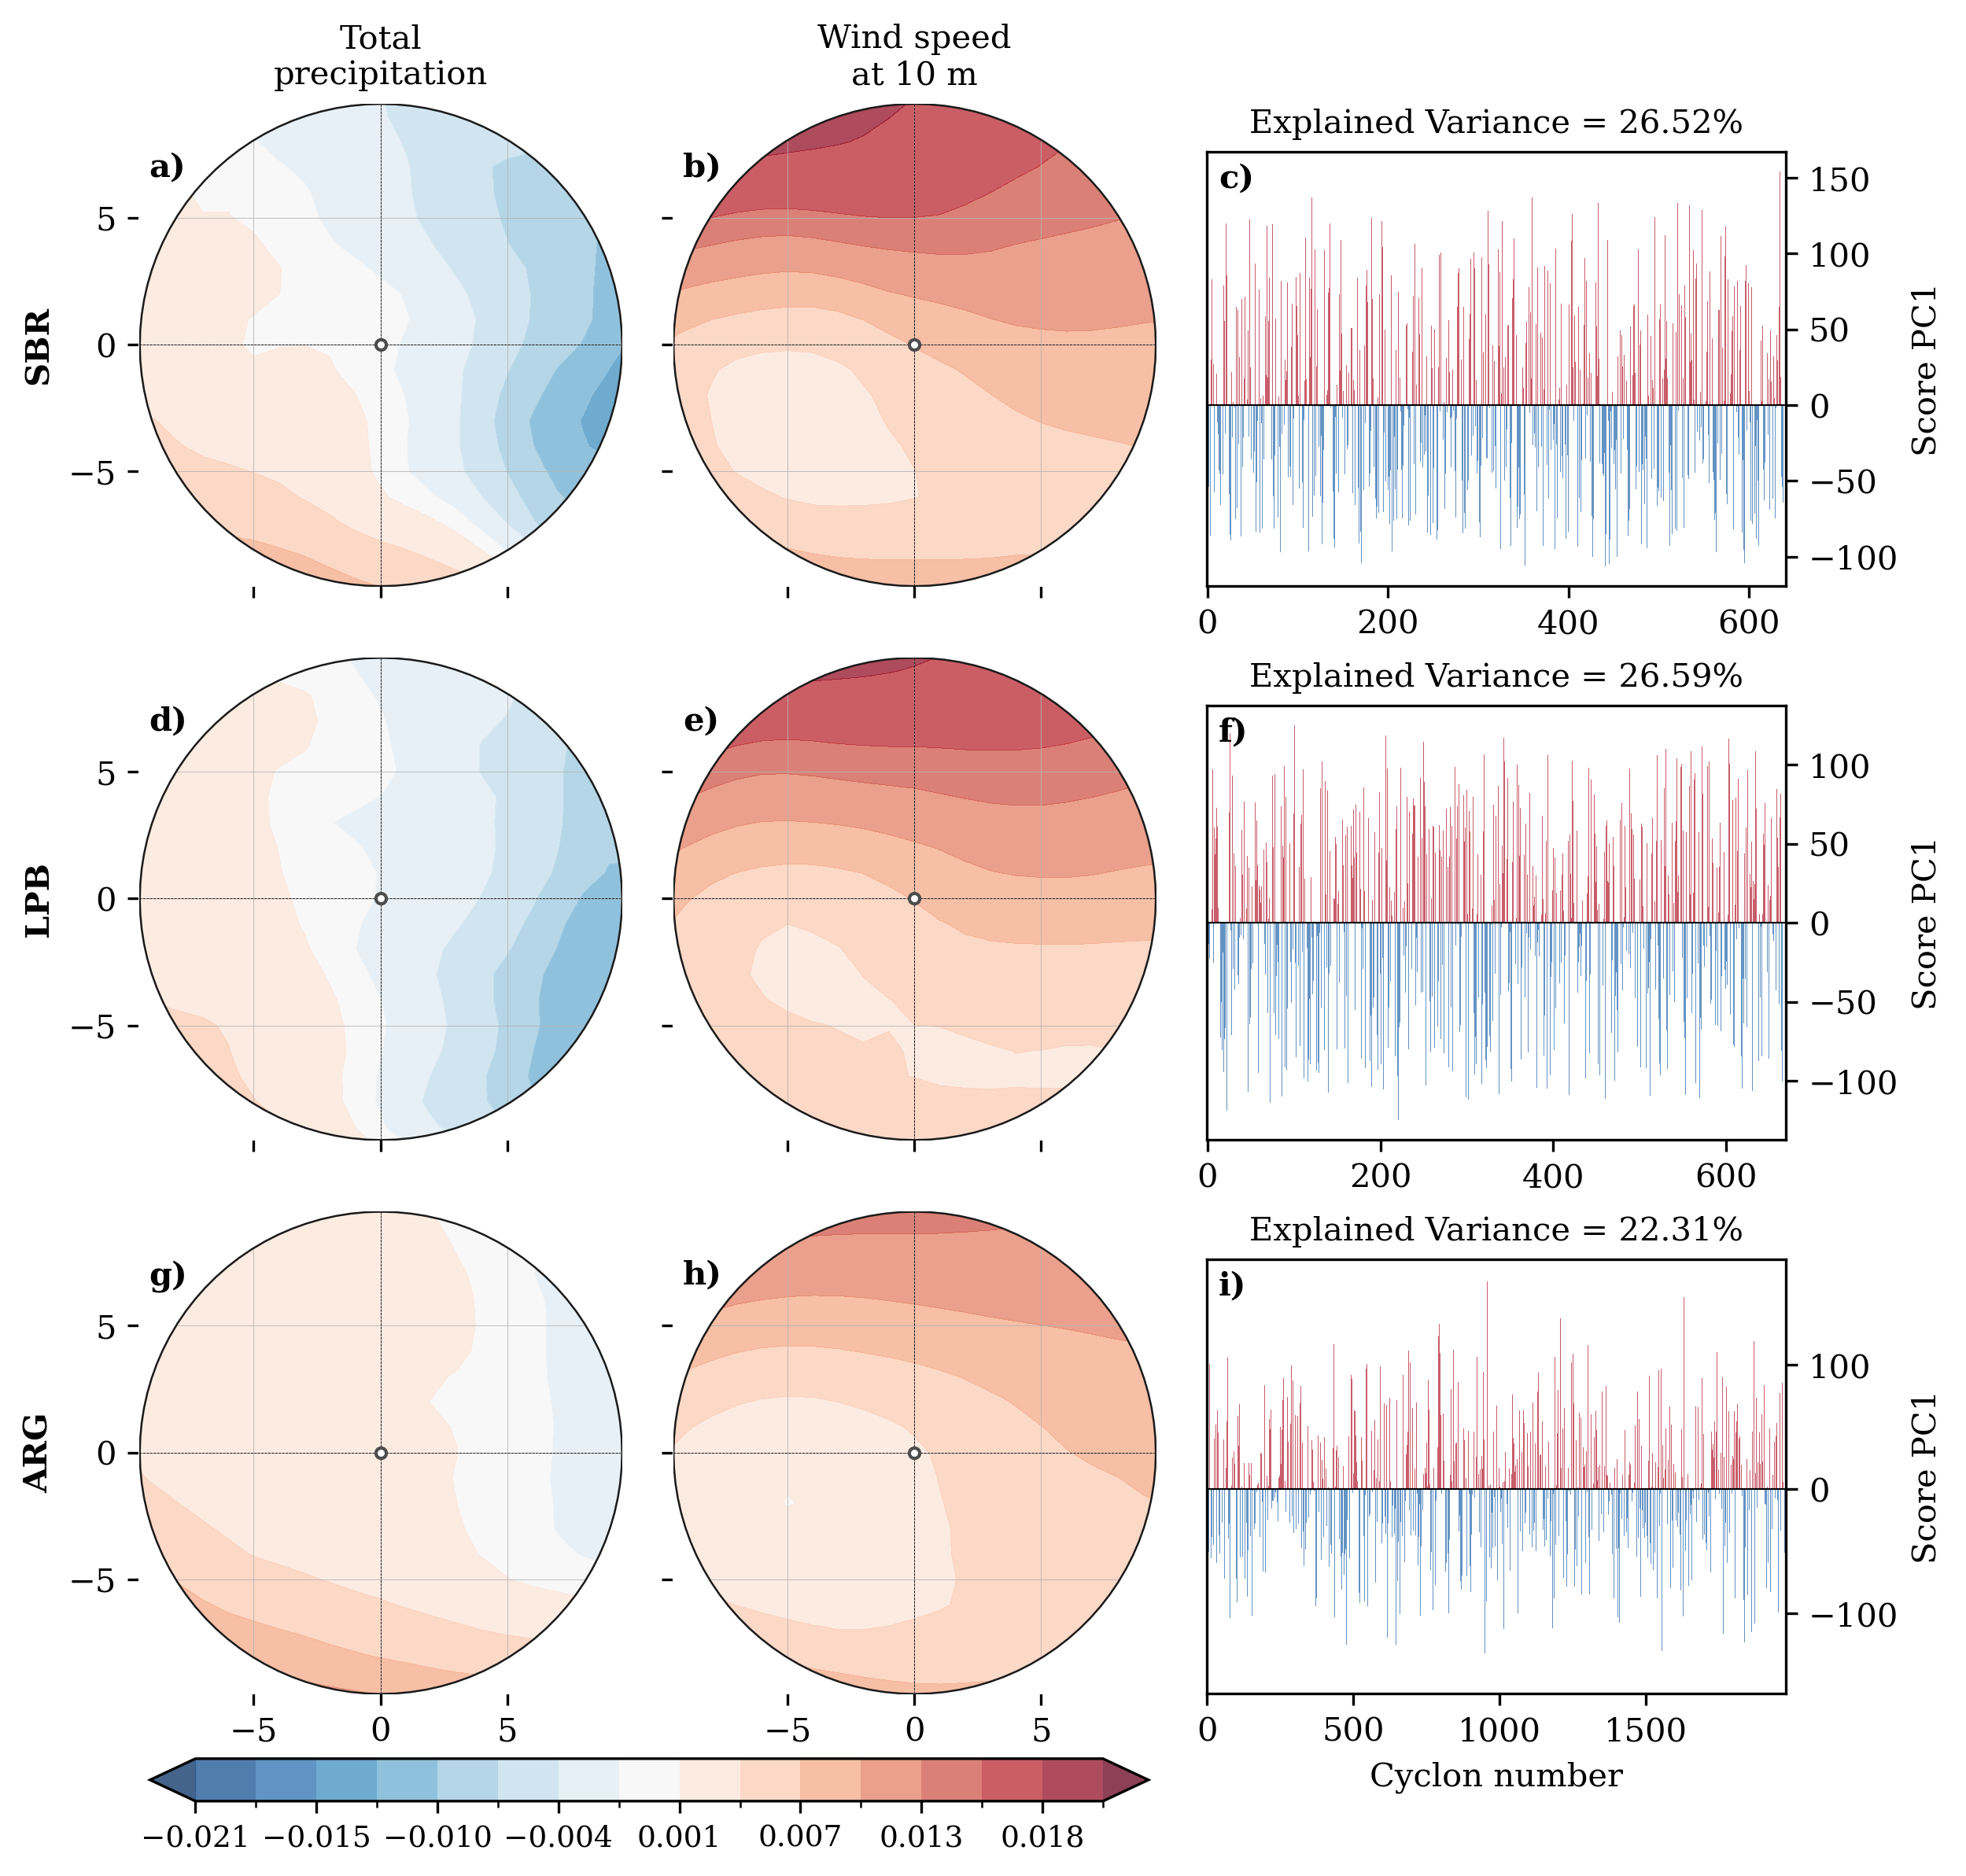
\includegraphics[width=\textwidth]{images/meof/meof1_mature_global.png}
    \caption[MEOF1 de vento a 10 m e precipitação -- Maturidade (População Global)]{Primeiro modo espacial multivariado (MEOF1) correspondente à fase de maturidade para a População Global. A disposição de painéis é idêntica às figuras precedentes. Documenta-se o padrão de covariabilidade de grande escala que caracteriza o ciclone ordinário em sua máxima intensidade, estabelecendo a linha de base em relação à qual se avalia a transformação estrutural do subconjunto de alta vorticidade.}
    \label{fig:meof_madurez_global}
\end{figure}

A Figura~\ref{fig:meof_madurez_p90} apresenta a matriz de cargas espaciais do MEOF1 para o subconjunto de alta vorticidade (p90) na fase de maturidade.

Com disposição idêntica de painéis, esta figura constitui o núcleo do capítulo. Seu propósito é mostrar a reorganização espacial entre os campos de precipitação e vento nos sistemas p90 do Atlântico Sul. O fato de cada componente univariada ser significativa separadamente (Seções~\ref{subsec:res_significancia_madurez} e~\ref{subsec:significancia_tp}) não garante que o modo conjunto também o seja. Não se conta com uma reamostragem Bootstrap-t multivariada independente para esta figura; essa limitação é retomada mais adiante (Seção~\ref{sec:discusion_meof}), ao mostrar que o modo conjunto às vezes reflete majoritariamente um único campo.
A variância conjunta explicada cai para 15.41\% (ARG), 16.42\% (LPB) e 19.02\% (SBR), muito abaixo dos valores da População Global na mesma fase, e também abaixo do EOF1 univariado de cada campo separadamente em p90-maturidade (vento: 25.4--37.6\%, Seção~\ref{sec:var_exp_wind10}; precipitação: 16--21.4\%, Seção~\ref{subsec:var_exp_tp}). O modo conjunto não é apenas menos dominante do que na População Global, mas menor do que qualquer um dos dois campos separadamente, consistente com o fato de ambos os campos se organizarem em setores geometricamente distintos do domínio (Figura~\ref{fig:meof_madurez_p90}), de modo que um único autovetor não pode capturar ambos os padrões com a mesma eficiência com que cada EOF univariado captura o seu. Essa separação, não a variância explicada, é o sinal que o MEOF permite identificar, e não uma limitação do método. Essa mesma ordem regional (SBR $>$ LPB $>$ ARG) já apareceu na concentração de magnitude e na densidade espacial dos máximos de vento (Seção~\ref{sec:kde_espacial_p90}), a terceira vez que se repete com um método distinto, agora em nível multivariado.

O contraste com a figura precedente é o mais marcado do capítulo.
O campo de precipitação (painéis a, d, g) exibe nas três regiões uma estrutura em arco compacta de anomalias positivas concentrada no quadrante sudeste e sul do domínio, com cargas que alcançam $+0.018$ em SBR (painel a) e $+0.015$ em LPB (painel d), indicando que o modo captura um padrão de precipitação localizado e recorrente nesse setor específico. Em SBR, o arco de precipitação (painel a) parte do sul e se estende em direção ao leste e nordeste.
Em LPB (painel d), a faixa é mais larga e se estende do quadrante sul até o leste, com o pico de carga deslocado em direção ao sudeste ($\Delta x \approx +3^{\circ}$, $\Delta y \approx -3^{\circ}$). Em ARG (painel g), o padrão de precipitação é o mais difuso dos três, com cargas positivas distribuídas no sudeste-sul mas com gradientes mais suaves.
O campo de vento (painéis b, e, h) apresenta uma configuração oposta. As anomalias positivas se concentram em um núcleo compacto a oeste do centro, aproximadamente na sua mesma latitude, com cargas que alcançam $+0.013$ em SBR (painel b) e $+0.010$ em LPB (painel e).
Esse núcleo de vento a oeste e o arco de precipitação a sudeste não apenas não compartilham setor, mas no domínio centrado no sistema se localizam em lados opostos em relação ao centro do vórtice (0,0).

\begin{figure}[htbp]
    \centering
    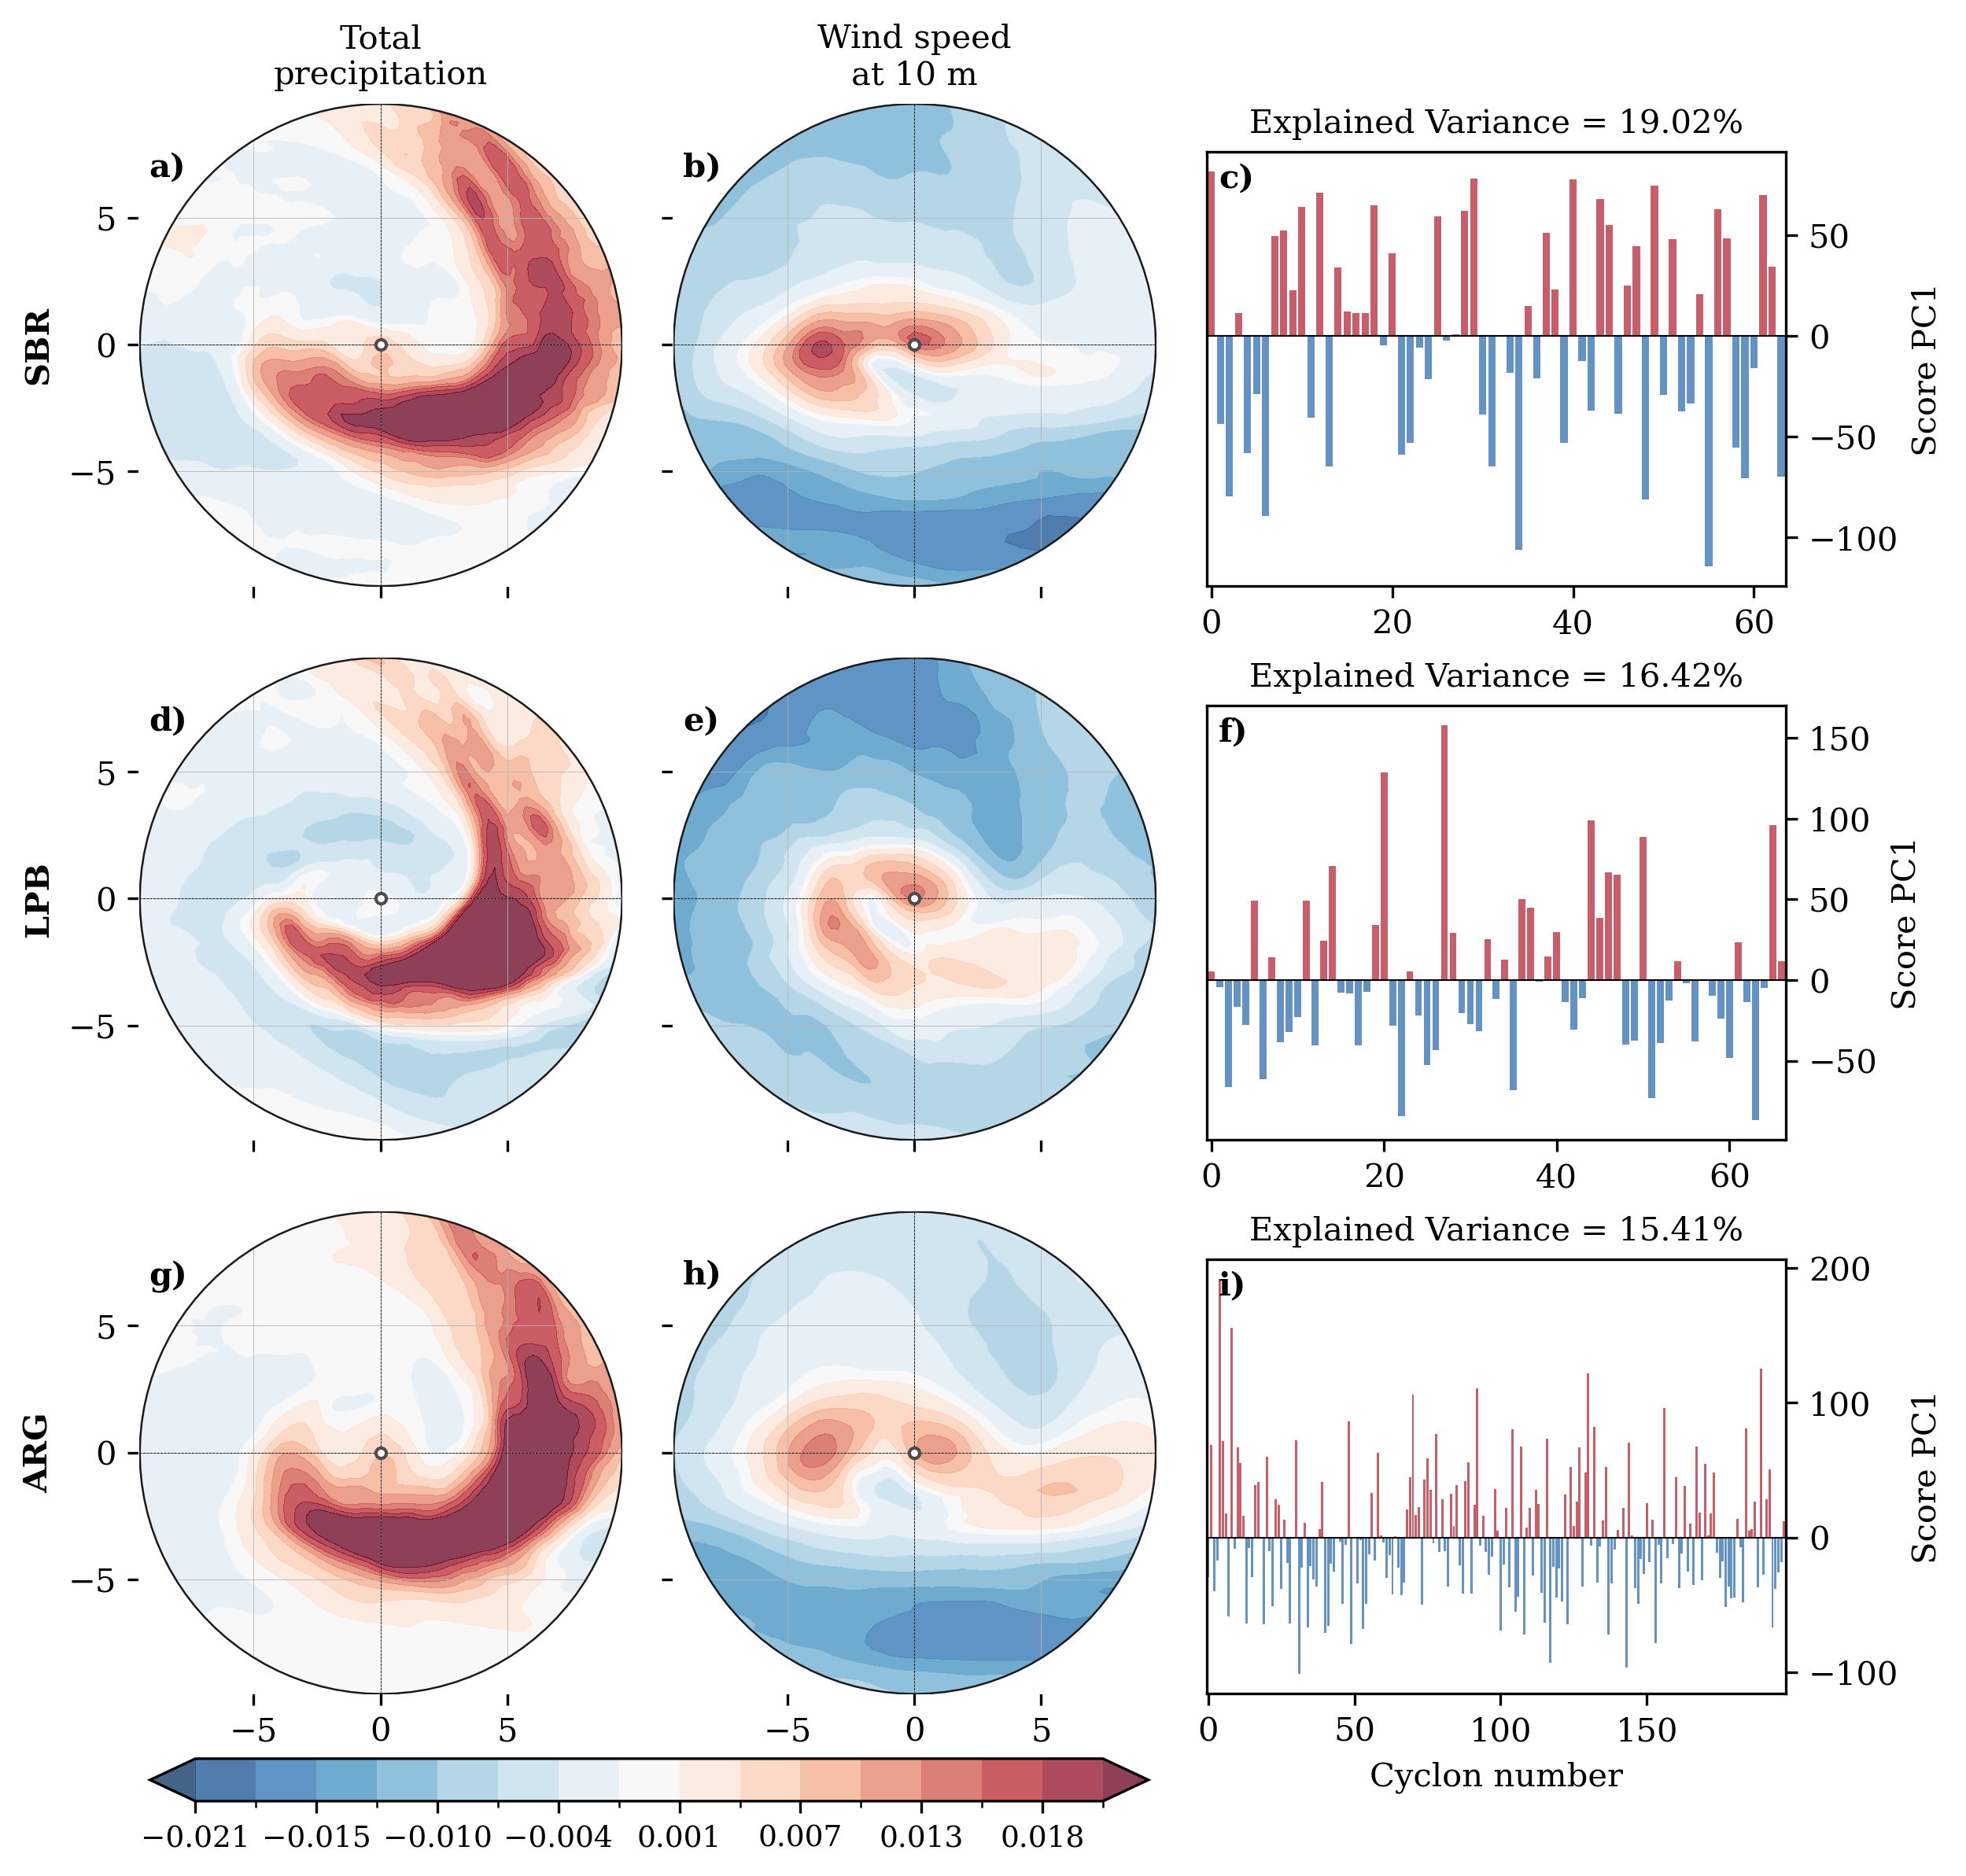
\includegraphics[width=\textwidth]{images/meof/meof1_mature_p90.png}
    \caption[MEOF1 de vento a 10 m e precipitação -- Maturidade (p90)]{Primeiro modo espacial multivariado (MEOF1) correspondente à fase de maturidade para o subconjunto de ciclones de alta vorticidade (p90). A disposição de painéis, a escala cromática e o domínio são idênticos às figuras precedentes.
Evidencia-se a reorganização espacial entre a banda de precipitação periférica no quadrante sudeste e o núcleo de vento a oeste do vórtice, a separação em quadrantes opostos que caracteriza os sistemas p90 do Atlântico Sul nessa fase.}
    \label{fig:meof_madurez_p90}
\end{figure}

A configuração de setores opostos documentada no MEOF1 de maturidade do subconjunto p90 é a evidência multivariada que integra e é coerente com os resultados dos capítulos precedentes.
O arco de precipitação sudeste capturado pelo MEOF1 corresponde à estrutura em arco periférica cuja assinatura PDFe foi documentada na Seção~\ref{subsec:kde_tp_p90} e cuja concentração de variância foi quantificada no EOF1 univariado (Seção~\ref{subsec:var_exp_tp}).
O núcleo de vento a oeste do MEOF1 coincide parcialmente com a concentração espacial identificada no PDFe de vento p90 (Seção~\ref{sec:kde_espacial_p90}) e com a estrutura compacta do EOF1 univariado de vento (Seção~\ref{subsec:eof1_wind10_p90}); embora ambos coincidam no setor ocidental, o núcleo de alta densidade da análise univariada se localiza no quadrante noroeste ($\Delta y \approx +2^{\circ}$ a $+3^{\circ}$), enquanto no MEOF1 o núcleo se localiza praticamente na mesma latitude do vórtice ($\Delta y \approx 0^{\circ}$), um deslocamento em direção ao sul sem causa determinada, que poderia se dever tanto à covariância com a precipitação quanto a um artefato da decomposição conjunta (Seção~\ref{sec:discusion_meof}). A novidade que o MEOF traz é que, ao decompor a covariância conjunta, mostra que a separação entre ambos os campos não é a justaposição acidental de dois padrões independentes, mas uma configuração geométrica estruturalmente coerente. O MEOF1 a captura como um único modo multivariado, o que indica que a precipitação ao sudeste e o vento a oeste covariam nos mesmos eventos, constituindo o padrão conjunto dominante da estrutura no Atlântico Sul.

A interpretação física dessa reorganização espacial poderia estar relacionada ao modelo de ciclone ocluso de Shapiro-Keyser. Em um ciclone do Hemisfério Norte com seclusão quente, \citet{shapiro1999bridge} documenta subsidência a oeste do centro, o que seria compatível com o fato de o núcleo de vento a oeste capturado pelo MEOF1 coincidir com ar mais seco e menos convectivo do que o setor sudeste, onde se concentra a precipitação. Em ciclones do Hemisfério Norte documentam-se ainda ventos extremos associados ao \textit{sting jet} e ao jato da cinta transportadora fria (CCB), situado abaixo e atrás dele \citep{clark2005sting, clark2018sting}, duas estruturas difíceis de distinguir em superfície por sua proximidade no espaço e no tempo \citep{eisenstein2023identification}; pela inversão da circulação entre hemisférios, esse setor corresponderia ao quadrante ocidental no Hemisfério Sul, coerente com a localização do núcleo de vento do MEOF1. Essa interpretação se apoia em estudos do Hemisfério Norte e em um caso único (Shapiro 1999), sem verificação direta para o Atlântico Sul.

\section{Coerência entre os Modos de Vento e Precipitação}
\label{sec:meof_coherencia}

Para confirmar se a reorganização espacial observada nos padrões do MEOF1 se traduz também em uma relação entre os dois campos em nível de eventos individuais, analisa-se a correlação entre as Componentes Principais univariadas de cada campo ($\text{PC1}^{\text{precip}}$ e $\text{PC1}^{\text{vento}}$), seguindo a metodologia descrita na Seção~\ref{subsec:analisis_pc}. Os resultados são apresentados na Tabela~\ref{tab:meof_coherencia}, que quantifica a evolução dessa relação ao longo do ciclo de vida para ambas as populações, com o fim de determinar se a separação espacial dos campos implica também que os ciclones que mais projetam sobre um padrão tendem a projetar menos sobre o outro.

\begin{table}[htbp]
\centering
\caption[Coerência entre os modos de precipitação e vento a 10m (Global e p90)]{Correlação de Spearman em valor absoluto ($|r|$) entre a PC1 de precipitação e a PC1 do vento a 10 metros, e seu valor de significância (\textit{p-valor}), para a População Global e o subconjunto extremo (p90). Reporta-se o valor absoluto porque cada PC1 provém de uma decomposição EOF univariada independente, com sua própria convenção de sinal arbitrária (Seção~\ref{subsec:analisis_pc}). Os valores em negrito indicam correlações estatisticamente significativas ($p < 0.05$).}
\label{tab:meof_coherencia}
\begin{tabular*}{\textwidth}{@{\extracolsep{\fill}}llrrrr}
\hline
\textbf{Região} & \textbf{Fase} & \multicolumn{2}{c}{\textbf{População Global}} & \multicolumn{2}{c}{\textbf{Subconjunto p90}} \\
\cline{3-4} \cline{5-6}
 & & \textbf{$|r|$} & \textbf{p-valor} & \textbf{$|r|$} & \textbf{p-valor} \\
\hline
\textbf{SBR} & Incipiente & \textbf{0.31} & $<$ 0.001 & \textbf{0.32} & 0.009 \\
 & Intensificação & \textbf{0.39} & $<$ 0.001 & 0.01 & 0.946 \\
 & Maturidade & \textbf{0.19} & $<$ 0.001 & \textbf{0.45} & $<$ 0.001 \\
 & Decaimento & \textbf{0.19} & $<$ 0.001 & 0.07 & 0.571 \\
\hline
\textbf{LPB} & Incipiente & \textbf{0.25} & $<$ 0.001 & 0.13 & 0.285 \\
 & Intensificação & \textbf{0.35} & $<$ 0.001 & 0.06 & 0.648 \\
 & Maturidade & \textbf{0.08} & 0.029 & \textbf{0.37} & 0.002 \\
 & Decaimento & \textbf{0.08} & 0.032 & 0.12 & 0.314 \\
\hline
\textbf{ARG} & Incipiente & \textbf{0.18} & $<$ 0.001 & 0.03 & 0.647 \\
 & Intensificação & \textbf{0.47} & $<$ 0.001 & 0.08 & 0.236 \\
 & Maturidade & \textbf{0.44} & $<$ 0.001 & \textbf{0.31} & $<$ 0.001 \\
 & Decaimento & \textbf{0.23} & $<$ 0.001 & \textbf{0.35} & $<$ 0.001 \\
\hline
\end{tabular*}
\end{table}


Na População Global, as correlações entre $\text{PC1}^{\text{precip}}$ e $\text{PC1}^{\text{vento}}$ são significativas durante as fases iniciais nas três regiões (Tabela~\ref{tab:meof_coherencia}), com magnitudes que oscilam entre $|r|=0.18$ e $0.47$. Em SBR e LPB, a correlação perde magnitude até a maturidade e o decaimento, embora se mantenha significativa ($|r|=0.19$ e $0.08$, respectivamente). Em ARG, por sua vez, a correlação se mantém significativa durante todo o ciclo de vida, alcançando seu máximo na intensificação ($|r|=0.47$) e mantendo-se quase igualmente forte na maturidade ($|r|=0.44$) antes de se atenuar no decaimento ($|r|=0.23$).

A correlação entre PC1 de precipitação e PC1 de vento durante a maturidade em p90 é significativa e de magnitude moderada nas três regiões ($|r| = 0.45$ em SBR, $0.37$ em LPB e $0.31$ em ARG). Esses dois índices provêm de decomposições EOF univariadas independentes (precipitação, Capítulo~\ref{cap:resultados_tp}; vento, Capítulo~\ref{cap:resultados_wind10}), cada uma com sua própria convenção de sinal arbitrária. Nessa fase e população, o núcleo positivo do EOF1 de precipitação se localiza a leste-sudeste e o do EOF1 de vento a oeste nas três regiões (Seções~\ref{subsec:eof1_tp_p90} e~\ref{subsec:eof1_wind10_p90}); com essa referência espacial verificada, o sinal observado indica que os ciclones com maior projeção sobre o núcleo sudeste de precipitação tendem a ter uma projeção menor ou nula sobre o núcleo ocidental de vento, e vice-versa, consistente com a separação em quadrantes opostos documentada no MEOF para essa mesma fase e população. No decaimento, SBR e LPB perdem significância ($|r|=0.07$ e $0.12$), enquanto ARG mantém uma correlação significativa de magnitude semelhante à da maturidade ($|r|=0.35$); essa persistência em magnitude é consistente com a maior dominância de seu EOF1 já apontada (Seção~\ref{subsec:pc1_global_tp}).

\section{Discussão}
\label{sec:discusion_meof}
% ==============================================================================

Os resultados da análise MEOF revelam uma transição qualitativa na relação espacial entre vento e precipitação que não é detectável mediante a análise univariada de cada variável separadamente.
Nos ciclones da População Global, o MEOF1 captura um padrão de covariância simples e extenso onde vento e precipitação permanecem majoritariamente positivos em todo o domínio centrado no sistema, sem núcleos isolados nem mudanças de sinal abruptas, com uma variância conjunta explicada entre 14.8\% e 26.6\%. Essa configuração reflete o desenvolvimento baroclínico clássico do modelo norueguês de frentes \citep{bjerknes1922life}, sistematizado posteriormente no marco do WCB como estrutura termodinâmica única que organiza a ascensão úmida (precipitação) e o fluxo de baixo nível (vento) no setor quente do ciclone \citep{browning1986conceptual}.
A suavidade e a extensão compartilhada das cargas MEOF1 de ambas as variáveis, embora orientadas em eixos distintos (oeste-leste em precipitação, norte-sul em vento), é a expressão quantitativa de que, no regime médio, os dois campos são manifestações do mesmo forçante sinótico e operam como uma estrutura dinâmica comum, sem que isso implique uma co-localização geométrica estrita.

A transição para o subconjunto p90 introduz uma mudança de regime que não pode ser atribuída a uma mera amplificação do padrão global.
A queda da variância conjunta explicada (de ${\sim}$26.6\% para ${\sim}$11.65--23.47\%) e a emergência de padrões de anticovariância entre precipitação e vento já durante a intensificação indicam que os ciclones p90 desenvolvem uma arquitetura multivariada diferente desde antes de alcançar sua maturidade.
Esse resultado é coerente com a classificação de \citet{corner2025classification}, que mostram mediante análise de componentes principais dispersas que as métricas dinâmicas dos ciclones mais intensos do Atlântico Norte e Europa não escalam linearmente com as métricas de impacto (precipitação, pegada de vento, severidade), mas exibem uma multidimensionalidade que requer várias medidas independentes para ser caracterizada.
No Hemisfério Sul, o MEOF fornece evidência equivalente mas no espaço da covariância espacial conjunta. O modo dominante já não captura um padrão simples e extenso, mas a geometria de separação entre os dois campos dinâmicos.

Um pressuposto central do MEOF é que o modo dominante reflete covariabilidade genuína entre ambos os campos, não a estrutura individual de um deles. \citet{bretherton1992intercomparison} advertem que essa abordagem pode se enviesar em direção ao EOF dominante de um único campo quando a razão sinal-ruído é baixa ou o tamanho amostral é reduzido (Seção~\ref{subsec:tb_eof}). Para avaliar esse risco, calculou-se a correlação espacial entre a carga de cada campo dentro do MEOF1 e o padrão de seu próprio EOF1 univariado, na mesma região, fase e população (Tabela~\ref{tab:meof_bias_check}, e Tabela~\ref{tab:meof_bias_check_completa} do Apêndice~\ref{apendice:meof_bias} para as quatro fases; o sinal de cada EOF é uma convenção independente e arbitrária entre decomposições distintas, por isso se reporta o valor absoluto).

\begin{table}[htbp]
\centering
\caption[Correlação espacial entre o MEOF1 e os EOF1 univariados (Global e p90)]{Correlação espacial (valor absoluto, $|r|$) entre a carga de cada campo dentro do MEOF1 e o padrão de seu próprio EOF1 univariado (vento a 10 m, Seção~\ref{sec:var_exp_wind10}; precipitação, Seção~\ref{subsec:var_exp_tp}), para a População Global e o subconjunto p90, nas fases incipiente e maturidade. As fases de intensificação e decaimento são apresentadas na Tabela~\ref{tab:meof_bias_check_completa} (Apêndice~\ref{apendice:meof_bias}).}
\label{tab:meof_bias_check}
\begin{tabular*}{\textwidth}{@{\extracolsep{\fill}}llrrrr}
\hline
\textbf{Região} & \textbf{Fase} & \multicolumn{2}{c}{\textbf{População Global}} & \multicolumn{2}{c}{\textbf{Subconjunto p90}} \\
\cline{3-4} \cline{5-6}
 & & \textbf{$|r|$ vento} & \textbf{$|r|$ precip.} & \textbf{$|r|$ vento} & \textbf{$|r|$ precip.} \\
\hline
\textbf{SBR} & Incipiente & 0.99 & 0.83 & 0.99 & 0.74 \\
 & Maturidade & 1.00 & 0.55 & 0.99 & 0.94 \\
\hline
\textbf{LPB} & Incipiente & 0.99 & 0.94 & 0.99 & 0.25 \\
 & Maturidade & 1.00 & 0.33 & 0.94 & 0.97 \\
\hline
\textbf{ARG} & Incipiente & 1.00 & 0.56 & 1.00 & 0.49 \\
 & Maturidade & 0.99 & 0.79 & 0.94 & 0.97 \\
\hline
\end{tabular*}
\end{table}


A carga de vento do MEOF1 coincide quase por completo com seu EOF1 univariado em praticamente todas as combinações de região, fase e população ($|r|>0.94$), tanto na População Global quanto em p90, exceto no decaimento de p90 para SBR ($|r|=0.26$) e LPB ($|r|=0.71$), onde o vento se debilita notavelmente. A carga de precipitação é muito mais variável. Na População Global flutua entre $|r|=0.33$ e $0.95$ sem uma tendência clara por fase ou região. Em p90, por sua vez, o padrão é mais definido: fraco em incipiente e intensificação em SBR e LPB ($|r|=0.08$ a $0.25$), e forte e consistente desde a maturidade nas três regiões ($|r|=0.85$ a $1.00$); ARG se mantém alto desde a intensificação ($|r|\geq0.92$). Isso indica que o vento ancora o MEOF1 em quase todas as combinações, e que a precipitação contribui com covariância genuína de forma mais sistemática em p90 a partir da maturidade do que na População Global, onde sua contribuição é mais errática. Essa leitura é consistente com a interpretação de viés em direção ao vento como regra geral, embora não se possa descartar que a correlação mais baixa de precipitação em p90-incipiente reflita também a menor variância explicada pelo próprio EOF1 univariado de precipitação nessa fase (13.8--15.3\% frente a 16.0--21.4\% na maturidade; Seção~\ref{subsec:var_exp_tp}).

A configuração de quadrantes opostos documentada no MEOF1 de maturidade do subconjunto p90 permite, além disso, estabelecer uma hierarquia física dos processos envolvidos.
A estrutura em arco de precipitação no quadrante sudeste capturada pelo MEOF1 se localiza em uma posição mais próxima da do WCB do que da do quadrante ocluso que \citet{martin1999forcing} descreve para a corrente do trowal (Seção~\ref{subsec:kde_tp_p90}); a convecção embutida no WCB, documentada por \citet{oertel2021warm} em um ciclone do Atlântico Norte, poderia sustentar a intensidade pluviométrica localizada nesse setor.
A organização do vento no setor ocidental é consistente com a caracterização da CCB como principal motor da circulação de baixo nível na fase de oclusão, que \citet{martinez2014cold} documenta observacionalmente e que \citet{eisenstein2023identification} confirma em climatologias europeias (denominada CJ, \textit{cold jet}, no estudo original).

Essa configuração conjunta é consistente com o vínculo termodinâmico subjacente entre ambos os fluxos; \citet{schemm2014linkage} demonstraram mediante simulações que a cinta transportadora fria e o WCB não operam de maneira isolada, mas estão conectados dinamicamente mediante a geração de anomalias de vorticidade potencial na baixa e alta troposfera, orquestrando o desenvolvimento integral do ciclone extratropical.
A contribuição do MEOF no presente trabalho é mostrar que essas duas estruturas, documentadas separadamente na literatura, tendem a covariar nos ciclones p90 do Atlântico Sul. A presença da estrutura em arco de precipitação a sudeste vem acompanhada da presença do núcleo de vento a oeste dentro do mesmo evento, consistente com a separação em quadrantes opostos que caracteriza esses sistemas na região.
Um paralelismo independente dessa dissociação, embora obtido com uma abordagem de coocorrência de extremos compostos em vez de MEOF, é fornecido por \citet{portal2024linking} para o Mediterrâneo. Em suas conclusões, a probabilidade de extremos compostos de chuva e vento se maximiza na ascensão do WCB (${\sim}$7\% dos casos), enquanto a de extremos de vento e ondas se maximiza tanto sob a saída da intrusão seca quanto sob o próprio WCB (mais de 10\% dos casos), o que indica que, em uma bacia de dimensões e dinâmica muito distintas, o WCB não está associado exclusivamente a um único tipo de perigo composto.

SBR e LPB mostram a maior separação geométrica entre as cargas do MEOF1 de precipitação e vento. Em ARG, a separação é moderada, com cargas MEOF1 de precipitação mais difusas.

\section{Síntese}
\label{sec:sintesis_meof}

A análise multivariada do MEOF mostra que os ciclones p90 do Atlântico Sul desenvolvem uma arquitetura dinâmica assimétrica que difere da da População Global.

\paragraph{Dimensionalidade da covariabilidade.}
Na População Global, o MEOF1 captura entre 14.8\% e 26.6\% da covariância conjunta com um padrão simples onde ambas as variáveis permanecem positivas e variam suavemente em eixos distintos do domínio (oeste-leste em precipitação, norte-sul em vento). Nos sistemas de alta vorticidade (p90), a variância cai para 11.65\%--23.47\% e se distribui entre múltiplos modos. O vento ancora esse modo dominante em praticamente todas as combinações de região, fase e população ($|r|>0.94$ frente a seu próprio EOF1 univariado), exceto no decaimento de p90 em SBR e LPB, onde se debilita notavelmente. A precipitação é mais variável: em p90 contribui com covariância genuína sobretudo a partir da maturidade, enquanto na População Global sua contribuição é mais errática e não segue um padrão claro por fase (Seção~\ref{sec:discusion_meof}).

\paragraph{Geometria da covariabilidade.}
O MEOF1 de maturidade do subconjunto p90 captura um padrão de anticovariância onde a precipitação e o vento se organizam em setores opostos do domínio centrado no sistema, com o arco de precipitação a sudeste e o núcleo de vento a oeste, possivelmente separados pela intrusão seca.

\paragraph{Coerência entre os campos.}
Essa separação geométrica é respaldada pela correlação significativa entre as PC1 univariadas de precipitação e vento durante a maturidade em p90 ($|r|$ entre $0.31$ e $0.45$, Seção~\ref{sec:meof_coherencia}), consistente com a separação em quadrantes opostos documentada no MEOF1. Isso indica que os sistemas p90 do Atlântico Sul não são a intensificação sincrônica de um único padrão frontal, mas a reorganização estrutural de dois campos dinâmicos que operam em setores diferenciados durante a maturidade.

\paragraph{Alcance.}
Esses resultados dependem da vorticidade de cada fase como medida pontual de intensidade, a mesma limitação apontada para os campos univariados \citep{sinclair1997objective}. A significância espacial do MEOF1 se apoia na de seus componentes univariados e não em uma reamostragem Bootstrap-t multivariada independente. Além disso, a interpretação da covariância conjunta como covariabilidade genuína depende de que ambos os campos contribuam com força comparável ao modo dominante, o que se cumpre com mais clareza em p90 a partir da maturidade e, de forma menos sistemática, em algumas combinações da População Global (Seção~\ref{sec:discusion_meof}); no restante dos casos, o MEOF1 é dominado quase por completo pelo vento. Finalmente, a interpretação mecanicista da separação em quadrantes opostos (WCB, CCB, intrusão seca) se apoia em estudos do Hemisfério Norte e do Mediterrâneo, sem uma comparação direta para o Atlântico Sul.

As bases físicas e estatísticas estabelecidas neste capítulo sustentam os protótipos estruturais apresentados no Capítulo~\ref{cap:prototipos}, onde os padrões EOF1 univariados de cada campo se integram com as densidades probabilísticas KDE para construir representações quantificadas da estrutura dinâmica por região e fase evolutiva, consistentes com a separação geométrica que o MEOF1 documenta mediante um modo de covariância conjunto.
